\section{Taxonomy}\label{sec:taxonomy}
% With the explosive growth of the number of LLMs, substantial LLMs have been adapted to code generation via continuing pre-training or fine-tuning, particularly for open-source models. 
% For example, LLaMA \cite{touvron2023llama} is first open-sourced by Meta AI, then subsequently releases the Code Llama \cite{roziere2023code}. 
% DeepSeek LLM \cite{bi2024deepseek}, developed by DeepSeeker, releases DeepSeek Coder \cite{guo2024deepseek}. 
% Qwen \cite{bai2023qwen}, developed by the Qwen team, released Code Qwen \cite{codeqwen}. 
% Microsoft releases WizardLM \cite{xu2023wizardlm} and then investigates the WizardCoder \cite{luo2023wizardcoder}.  
% Google also released Gemma \cite{team2024gemma} and then released Code Gemma \cite{codegemma_2024}. 
% In addition to extending existing general-purpose LLM for code generation, there are also substantial works specialized for code generation, such as StarCoder \cite{li2023starcoder}, OctoCoder \cite{muennighoff2023octopack}, and CodeGen \cite{nijkamp2022codegen}. 
The recent surge in the development of \done{LLMs} has led to a significant number of these models being repurposed for code generation task through continual pre-training or fine-tuning. 
This trend is particularly observable in the realm of open-source models. 
For instance, Meta AI initially made the LLaMA \cite{touvron2023llama} model publicly available, which was followed by the release of Code Llama \cite{roziere2023code}, designed specifically for code generation. 
Similarly, DeepSeek LLM \cite{bi2024deepseek} developed and released by DeepSeek has been extended to create DeepSeek Coder \cite{guo2024deepseek}, a variant tailored for code generation. 
The Qwen team has developed and released Code Qwen \cite{codeqwen}, building on their original Qwen \cite{bai2023qwen} model. 
Microsoft, on the other hand, has unveiled WizardLM \cite{xu2023wizardlm} and is exploring its coding-oriented counterpart, WizardCoder \cite{luo2023wizardcoder}. 
Google has joined the fray by releasing Gemma \cite{team2024gemma}, subsequently followed by Code Gemma \cite{codegemma_2024}.
Beyond simply adapting general-purpose LLMs for code-related tasks, there has been a proliferation of models specifically engineered for code generation. Notable examples include StarCoder \cite{li2023starcoder}, OctoCoder \cite{muennighoff2023octopack}, and CodeGen \cite{nijkamp2022codegen}. These models underscore the trend of LLMs being developed with a focus on code generation.

% Basically, the line of LLMs for code generation research follows the latest development of LLMs. 
% Thus, we introduce a taxonomy to categorize and examine recent advancements that serve as a foundational reference for researchers quickly exploring the latest progress in LLMs for code generation. Figure \ref{fig:taxonomy} illustrates our taxonomy and some representative LLMs for code generation.
Recognizing the importance of these developments, 
\done{we conduct a thorough analysis of selected papers on LLMs for code generation, sourced from widely used scientific databases as mentioned in Section \ref{sec:methodology}. 
Based on this analysis, we propose a taxonomy that categorizes and evaluates the latest advancements in LLMs for code generation.}
This taxonomy, depicted in Figure \ref{fig:taxonomy}, serves as a comprehensive reference for researchers seeking to quickly familiarize themselves with the state-of-the-art in this dynamic field.
\done{It is important to highlight that the category of recent advances emphasizes the core techniques used in the current state-of-the-art code LLMs.}

% In the following section, we will focus on delineating each item for code generation in detail, including the definition of the problem, the problem to be solved, and the comparison of currently represented models and performance.
In the subsequent sections, we will provide an in-depth analysis of each category related to code generation. This will encompass a definition of the problem, the challenges to be addressed, and a comparison of the most prominent models and their performance evaluation.

\begin{figure}[t]
\centering
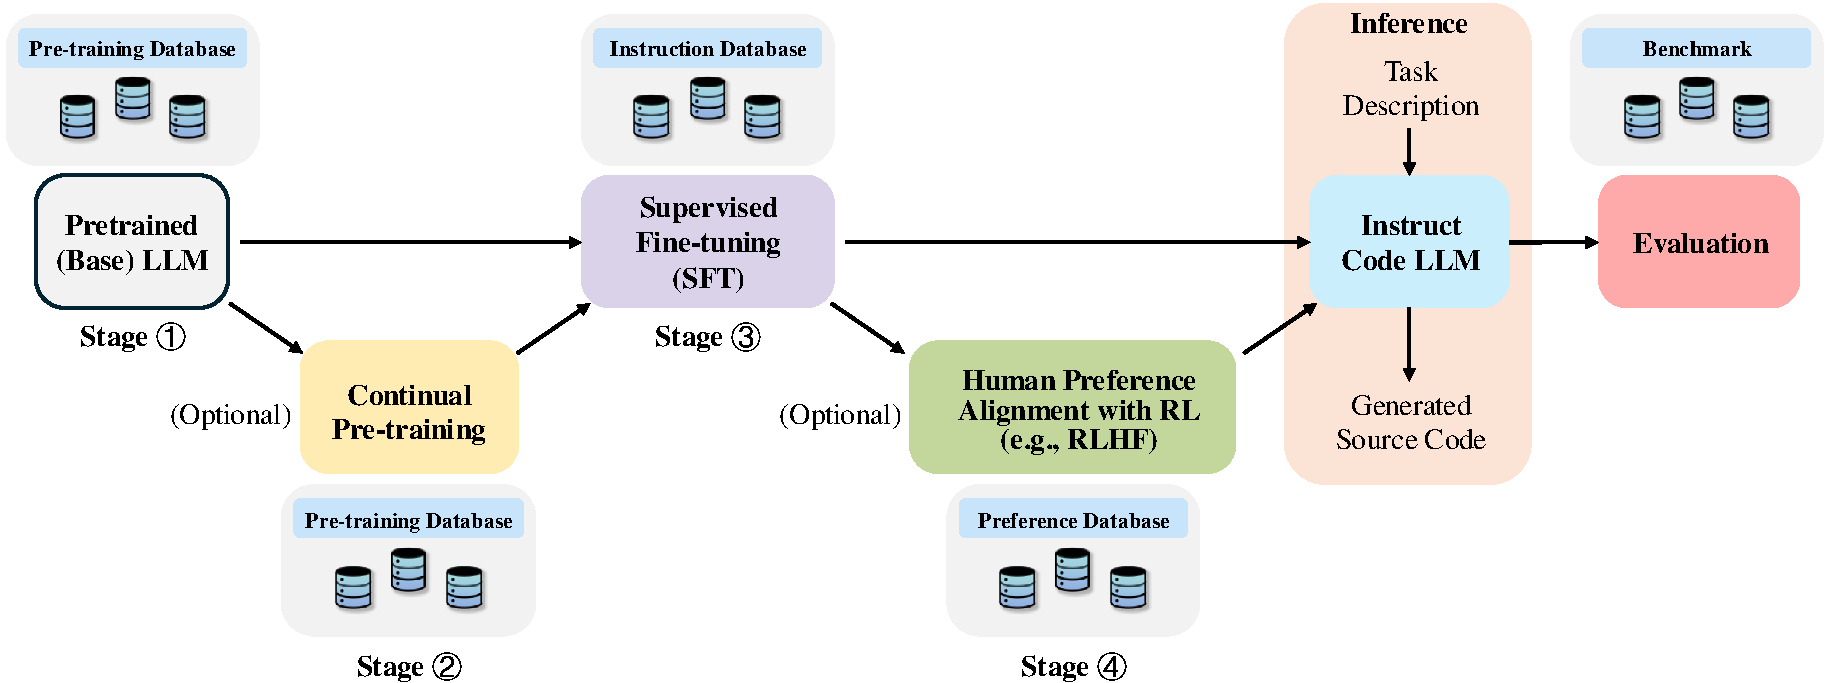
\includegraphics[width=0.95\linewidth]{images/codellm_workflow_v5.pdf}
\caption{\done{A diagram illustrating the general training, inference, and evaluation workflow for Code LLMs and their associated databases. 
The training workflow is mainly divided into four distinct stages: 
Stage \textcircled{1} and \textcircled{2} are the pre-training phase, whereas Stages \textcircled{3} and \textcircled{4} represent the post-training phases. It is important to note that Stage \textcircled{2} and \textcircled{4} are optional. 
For instance, StarCoder \cite{li2023starcoder} incorporates only Stage \textcircled{1}. WizardCoder \cite{luo2023wizardcoder}, fine-tuned upon StarCoder, includes only Stage \textcircled{3}, while Code Llama \cite{roziere2023code}, continually pre-trained on Llama 2, encompasses Stages \textcircled{2} and \textcircled{3}. DeepSeek-Coder-V2 \cite{zhu2024deepseek}, continually pre-trained on DeepSeek-V2, covers Stages \textcircled{2}, \textcircled{3}, and \textcircled{4}. 
Note that pre-trained model can be directly used for inference through prompt engineering.
}}
\label{fig:codellm_workflow}
\end{figure}

\definecolor{line-color}{RGB}{0, 119, 182}
\definecolor{fill-color}{RGB}{114, 200, 222}
\tikzstyle{category}=[
    rectangle,
    draw=line-color,
    rounded corners,
    text opacity=1,
    minimum height=1.5em,
    minimum width=5em,
    inner sep=2pt,
    align=center,
    fill opacity=.5,
]

\tikzstyle{leaf}=[category,minimum height=1em,
fill=fill-color!40, text width=20em,  text=black,align=left,font=\tiny,
inner xsep=2pt,
inner ysep=1pt,
]

\begin{figure*}[tp]
\centering
\scalebox{0.97}{
\begin{forest}
  forked edges,
  for tree={
  grow=east,
  reversed=true,%increase counter-clockwise
  anchor=base west,
  parent anchor=east,
  child anchor=west,
  base=left,
  font=\small,
  rectangle,
  draw=line-color,
  rounded corners,align=left,
  minimum width=2.5em,
  %  edge+={darkgray, line width=1pt},
%  l sep+=2.5pt,
%  s sep+=-5pt,
s sep=3pt,
inner xsep=2pt,
inner ysep=1pt,
%align=center,
ver/.style={rotate=90, child anchor=north, parent anchor=south, anchor=center},
  },
  %before packing={where n children=3{calign child=2, calign=child edge}{}},
  %before typesetting nodes={where content={}{coordinate}{}},
  %where level<=1{line width=2pt}{line width=1pt},
  where level=1{text width=3.2em,font=\scriptsize,}{},
  where level=2{text width=3.8em,font=\tiny}{},
  where level=3{text width=4.0em,font=\tiny}{},%yshift=0.26pt
  where level=4{text width=4.2em,font=\tiny}{},%yshift=0.26pt
  [LLMs for Code Generation, ver
    [Data \\Curation \\(Sec. \ref{sec:data_curation})
        [Pre-training
            [CodeSearchNet\cite{husain2019codesearchnet}{,}
             Google BigQuery\cite{hoffa2016github}{,}
             The Pile\cite{gao2020pile}{,}
             CodeParrot\cite{tunstall2022natural}{,}
             GitHub Code\cite{tunstall2022natural}\\
             ROOTS\cite{laurenccon2022bigscience}{,}
             The Stack\cite{kocetkov2022stack}{,}
             The Stack v2\cite{lozhkov2024starcoder}
            ,leaf,text width=24.5em]
        ]
        [Instruction \\Tuning
            [CommitPackFT \cite{muennighoff2023octopack}{,}
             Code Alpaca\cite{codealpaca}{,}
             OA-Leet\cite{oa-leet10k}{,}
             OSS-Instruct\cite{wei2023magicoder}{,}
             Evol-instruction\cite{evol_instruction}\\
             Self-OSS-Instruct-SC2-Exec-Filter\cite{starcoder2instruct}
            ,leaf,text width=24.5em]
        ]
        % [Alignment
        %     [
        %     ,leaf,text width=19.5em]
        % ]
        [Benchmarks
            [General
                [HumanEval\cite{chen2021evaluating}{,}
                 HumanEval+\cite{liu2024your}{,}
                 HumanEvalPack\cite{muennighoff2023octopack}{,}
                 MBPP\cite{austin2021program}\\
                 MBPP+\cite{liu2024your}{,}
                 CoNaLa\cite{yin2018learning}{,}
                 Spider\cite{yu2018spider}{,}
                 CONCODE\cite{iyer2018mapping}{,}
                 ODEX\cite{wang2022execution}\\
                 CoderEval\cite{yu2024codereval}{,}
                 ReCode\cite{wang2022recode}{,}
                 StudentEval\cite{babe2023studenteval}
                ,leaf,text width=19em]
            ]
            [Competitions
                [APPS\cite{hendrycks2021measuring}{,}
                 CodeContests\cite{li2022competition}
                ,leaf,text width=19em]
            ]
            [Data Science
                [DSP\cite{chandel2022training}{,}
                DS-1000\cite{lai2023ds}{,}
                ExeDS\cite{huang2022execution}
                ,leaf,text width=19em]
            ]
            [Multilingual
                [MBXP\cite{athiwaratkun2022multi}{,}
                 Multilingual HumanEval\cite{athiwaratkun2022multi}{,}
                 HumanEval-X\cite{zheng2023codegeex}{,}
                 MultiPL-E\cite{cassano2022scalable}\\
                 xCodeEval\cite{khan2023xcodeeval}
                ,leaf,text width=19em]
            ]
            [Reasoning
                [MathQA-X\cite{athiwaratkun2022multi}{,}
                 MathQA-Python\cite{austin2021program}{,}
                 GSM8K\cite{cobbe2021training}{,}
                 GSM-HARD\cite{gao2023pal}
                ,leaf,text width=19em]
            ]
            [Repository
                [RepoEval\cite{zhang2023repocoder}{,}
                 Stack-Repo\cite{shrivastava2023repofusion}{,} 
                 Repobench\cite{liu2023repobench}{,}
                 EvoCodeBench\cite{li2024evocodebench}\\
                 SWE-bench\cite{jimenez2023swe}{,}
                 CrossCodeEval\cite{ding2024crosscodeeval}{,}
                 SketchEval\cite{zan2024codes}
                ,leaf,text width=19em]
            ]
            % [
            %  % DSP
            %  % PandasEval\cite{zan2022cert}
            %  % NumpyEval\cite{zan2022cert}\\
            %  % TorchDataEval
            %  % MTPB
            %  % ODEX
            %  % BIG-Bench
            % ,leaf,text width=24.5em]
        ]
        % [Data \\Preprocessing
        %     [
        %     ,leaf,text width=24.5em]
        % ]
        % [Data \\Scheduling
        %     [
        %     ,leaf,text width=24.5em]
        % ]
    ]
    [Recent \\Advances
        % [Tokenization
        %     [WordPiece
        %         [
        %         ,leaf,text width=19.5em]
        %     ]
        %     [Byte-Pair \\Encoding
        %         [
        %         ,leaf,text width=19.5em]
        %     ]
        %     [Byte-level \\BPE
        %         [
        %         ,leaf,text width=19.5em]
        %     ]
        % ]
        [Data \\Synthesis \\(Sec. \ref{sec:data_synthesis})
            [Self-Instruct \cite{wang2023self}{,}
            Evol-Instruct \cite{xu2023wizardlm}{,}
            Phi-1\cite{gunasekar2023textbooks}{,}
            Code Alpaca\cite{codealpaca}{,}
            WizardCoder\cite{luo2023wizardcoder}\\
            Magicoder\cite{wei2023magicoder}{,}
            StarCoder2-instruct \cite{starcoder2instruct}
            ,leaf,text width=24.5em]
        ]
        [Pre-training \\(Sec. \ref{sec:pre-training})
            [Model \\Architectures
                [Encoder-Decoder
                    [PyMT5\cite{clement2020pymt5}{,}
                    PLBART\cite{ahmad2021unified}{,}
                    CodeT5\cite{wang2021codet5}{,}
                    JuPyT5\cite{chandel2022training}\\
                    AlphaCode\cite{li2022competition}{,}
                    CodeRL\cite{le2022coderl}{,}
                    ERNIE-Code\cite{chai2022ernie}\\
                    PPOCoder\cite{shojaee2023execution}{,}
                    CodeT5+\cite{wang2023codet5+}{,}
                    % CodeTF\cite{}
                    CodeFusion\cite{singh2023codefusion}\\
                    AST-T5\cite{gong2024ast}
                    ,leaf,text width=13em]
                ]
                [Decoder-Only
                    [GPT-C\cite{svyatkovskiy2020intellicode}{,}
                    GPT-Neo\cite{gpt-neo}{,}
                    GPT-J\cite{gpt-j}{,}
                    Codex\cite{chen2021evaluating}\\
                    CodeGPT\cite{lu2021codexglue}{,}
                    CodeParrot\cite{tunstall2022natural}{,}
                    PolyCoder\cite{xu2022systematic}\\
                    CodeGen\cite{nijkamp2022codegen}{,}
                    GPT-NeoX\cite{black2022gpt}{,}
                    PaLM-Coder\cite{chowdhery2023palm}\\
                    InCoder\cite{fried2022incoder}{,}
                    PanGu-Coder\cite{christopoulou2022pangu}{,}
                    PyCodeGPT\cite{zan2022cert}\\
                    CodeGeeX\cite{zheng2023codegeex}{,}
                    BLOOM\cite{le2023bloom}{,}
                    ChatGPT\cite{gpt-3.5-turbo}\\
                    SantaCoder\cite{allal2023santacoder}{,}
                    LLaMA\cite{touvron2023llama}{,}
                    GPT-4\cite{achiam2023gpt}\\
                    CodeGen2\cite{nijkamp2023codegen2}{,}
                    replit-code\cite{replit-code}{,}
                    StarCoder\cite{li2023starcoder}\\
                    WizardCoder\cite{luo2023wizardcoder}{,}
                    phi-1\cite{gunasekar2023textbooks}{,}
                    ChainCoder\cite{zheng2023outline}\\
                    CodeGeeX2\cite{zheng2023codegeex}{,}
                    PanGu-Coder2\cite{shen2023pangu}{,}
                    Llama 2\cite{touvron2023llama2}\\
                    OctoPack\cite{muennighoff2023octopack}{,}
                    Code Llama\cite{roziere2023code}{,}
                    MFTCoder\cite{liu2023mftcoder}\\
                    phi-1.5\cite{li2023textbooks}{,}
                    CodeShell\cite{xie2024codeshell}{,}
                    Magicoder\cite{wei2023magicoder}\\
                    AlphaCode 2\cite{alphacode2}{,} 
                    StableCode\cite{pinnaparaju2024stable}{,}
                    WaveCoder\cite{yu2023wavecoder}\\
                    phi-2\cite{phi-2}{,}
                    DeepSeek-Coder\cite{guo2024deepseek}{,}
                    StepCoder\cite{dou2024stepcoder}\\
                    OpenCodeInterpreter\cite{zheng2024opencodeinterpreter}{,}
                    StarCoder 2\cite{lozhkov2024starcoder}\\
                    Claude 3\cite{claude3}{,}
                    ProCoder\cite{bi2024iterative}{,}
                    CodeGemma\cite{codegemma_2024}\\
                    CodeQwen\cite{codeqwen}{,}
                    Llama3\cite{llama3}\\
                    StarCoder2-Instruct\cite{starcoder2instruct}{,}
                    Codestral\cite{codestral}
                    ,leaf,text width=13em]
                ]
            ]
            [Pre-training \\Tasks
                [CLM\cite{li2023starcoder,luo2023wizardcoder,wei2023magicoder,guo2024deepseek}{,} 
                DAE\cite{ahmad2021unified,wang2021codet5,wang2023codet5+}{,}
                Auxiliary\cite{wang2021codet5,chai2022ernie,wang2023codet5+} 
                ,leaf,text width=16.5em]
            ]
        ]
        [Fine-tuning
            [Instruction \\Tuning \\(Sec. \ref{sec:instruction_tuning})
                [Full Parameter\\ Fine-tuning
                    [Code Alpaca\cite{codealpaca}{,} 
                    CodeT5+\cite{wang2021codet5}{,} WizardCoder\cite{luo2023wizardcoder}\\ StarCoder\cite{li2023starcoder}{,} 
                    Pangu-Coder2\cite{shen2023pangu}{,} OctoPack\cite{muennighoff2023octopack}\\ CodeGeeX2\cite{zheng2023codegeex}{,} Magicoder\cite{wei2023magicoder}{,} CodeGemma\cite{codegemma_2024}\\ 
                    StarCoder2-instruct\cite{starcoder2instruct}
                    ,leaf,text width=13em]
                ]
                [Parameter \\Efficient \\Fine-tuning
                    [CodeUp\cite{codeup}{,} 
                    ASTRAIOS\cite{zhuo2024astraios}
                    ,leaf,text width=8em]
                ]
            ]
            [Reinforcement \\Learning \\with Feedback \\(Sec. \ref{sec:reinforcement_learning})
              [CodeRL\cite{le2022coderl}{,} 
              CompCoder\cite{wang2022compilable}{,} PPOCoder\cite{shojaee2023execution}{,} 
              RLTF\cite{liu2023rltf}\\
              PanGu-Coder2\cite{shen2023pangu}{,}
              StepCoder\cite{dou2024stepcoder}
                ,leaf,text width=15em]
            ]
        ]
        [Prompting \\Engineering \\(Sec. \ref{sec:prompting})
          [Reflexion\cite{shinn2024reflexion}{,} 
          LATS\cite{zhou2023language}{,} 
          Self-Debugging\cite{chen2023teaching}{,} 
          SelfEvolve\cite{jiang2023selfevolve}\\ 
          Theo X. et al.\cite{olausson2023self}{,} 
          CodeT\cite{chen2022codet}{,} 
          LEVER\cite{ni2023lever}{,}
          AlphaCodium\cite{ridnik2024code}
            ,leaf,text width=17em]
        ]
        [Repository\\ Level \& Long \\Context \\(Sec. \ref{sec:repository_level}) 
            [RepoCoder\cite{zhang2023repocoder}{,} 
            CoCoMIC\cite{ding2022cocomic}{,} 
            RepoHyper\cite{phan2024repohyper}{,} 
            RLPG\cite{shrivastava2023repository}\\
            Repoformer\cite{wu2024repoformer}{,} 
            RepoFusion\cite{shrivastava2023repofusion}{,} 
            ToolGen\cite{wang2024teaching}{,}
            CodePlan\cite{bairi2023codeplan}\\
            CodeS\cite{zan2024codes} 
            ,leaf,text width=17em]
        ]
        [Retrieval \\Augmented \\(Sec. \ref{sec:retrieval_augmented})
          [HGNN\cite{liu2020retrieval}{,} 
          REDCODER\cite{parvez2021retrieval}{,} 
          ReACC\cite{lu2022reacc}{,} 
          DocPrompting\cite{zhou2022docprompting}\\ 
          RepoCoder\cite{zhang2023repocoder}{,} 
          Su et al.\cite{su2024arks}
            ,leaf,text width=17em]
        ]
        [Autonomous \\Coding Agents \\(Sec. \ref{sec:autonomous_agents})
          [AgentCoder \cite{huang2023agentcoder}{,}
          MetaGPT\cite{hong2023metagpt}{,}
          CodeAct \cite{wang2024executable}{,}
          AutoCodeRover \cite{zhang2024autocoderover}{,}
          Devin\cite{Devin}\\
          OpenDevin\cite{OpenDevin}{,}
          SWE-agent\cite{swe-agent}{,}
          L2MAC\cite{holt2023l2mac}{,}
          OpenDevin CodeAct 1.0\cite{OpenDevin_CodeAct}
            ,leaf,text width=22em]
        ]
        % [Interpretability
        %   [
        %     ,leaf,text width=16em]
        % ]
    ]
    [Evaluation \\(Sec. \ref{sec:evaluation})
        [Metrics
            [Exact Match{,} 
            BLEU\cite{papineni2002bleu}{,} 
            ROUGE\cite{lin2004rouge}{,}
            METEOR\cite{banerjee2005meteor}{,}
            CodeBLEU\cite{ren2020codebleu}{,}
            pass@k\cite{chen2021evaluating}\\
            n@k\cite{li2022competition}{,}
            test case average\cite{hendrycks2021measuring}{,}
            execution accuracy\cite{rajkumar2022evaluating}{,}
            pass@t\cite{olausson2023self}{,}
            perplexity\cite{jelinek1977perplexity}
            ,leaf,text width=22em]
        ]
        [Human \\Evaluation
            [CodePlan\cite{bairi2023codeplan}{,} 
            RepoFusion\cite{shrivastava2023repofusion}{,}
            CodeBLEU\cite{ren2020codebleu}
            ,leaf,text width=13em]
        ]
        [LLM-as-a-Judge
            [AlpacaEval\cite{alpaca_eval}{,}
            MT-bench\cite{zheng2024judging}{,}
            ICE-Score\cite{zhuo2024ice}
            ,leaf,text width=13em]
        ]
    ]
    [\textcolor{black}{Code LLMs} \\\textcolor{black}{Alignment} \\(Sec. \ref{sec:grest_llm4code})
      [\textcolor{black}{Green\cite{shi2024greening,wei2023towards}{,}}
      \textcolor{black}{Responsibility\cite{liu2023uncovering,xu2024first}{,}}
      \textcolor{black}{Efficiency\cite{yang2024robustness}{,}}
      \textcolor{black}{Safety\cite{schuster2021you,hajipour2024codelmsec,yang2024unveiling,al2024traces,yuan2023gpt,fried2022incoder,allal2023santacoder}{,}}
      \textcolor{black}{Trustworthiness\cite{ji2023benchmarking,palacio2023evaluating}}
        ,leaf,text width=29.8em]
    ]
    % [Inference \\(Decoding)
    %     [Deterministic
    %         [Greedy Search{,} Beam Search
    %         ,leaf,text width=22em]
    %     ]
    %     [Sampling
    %         [Temperature Sampling{,} Top-k Sampling{,} Top-p Sampling
    %         ,leaf,text width=22em]
    %     ]
    %     [Speculative \\Decoding
    %         [
    %         ,leaf,text width=22em]
    %     ]
    % ]
    [Application \\(Sec. \ref{sec:application})
        [GitHub Copilot\cite{chen2021evaluating}{,} 
        CodeGeeX\cite{zheng2023codegeex}{,} 
        CodeWhisperer\cite{CodeWhisperer}{,} 
        Codeium\cite{Codeium}{,} 
        CodeArts Snap\cite{shen2023pangu}{,} 
        TabNine\cite{TabNine}{,} 
        Replit\cite{Replit}
         ,leaf,text width=29.8em]
    ]
  ]
\end{forest}
}
\caption{Taxonomy of \done{LLMs} for code generation.}
\label{fig:taxonomy}
\end{figure*}